\documentclass[11pt,a4paper]{article}

%opening
\title{¡Hola mundo!}
\author{Mihdí Caballero}

\usepackage[spanish]{babel}
\usepackage{graphicx}
\usepackage{mathtools}

\begin{document}

\maketitle

\begin{abstract}
hola
\end{abstract}

\section{Título de sección}
Texto de primer párrafo.

\newpage 
Texto de primer párrafo.
\begin{figure}[h]
	\centering
	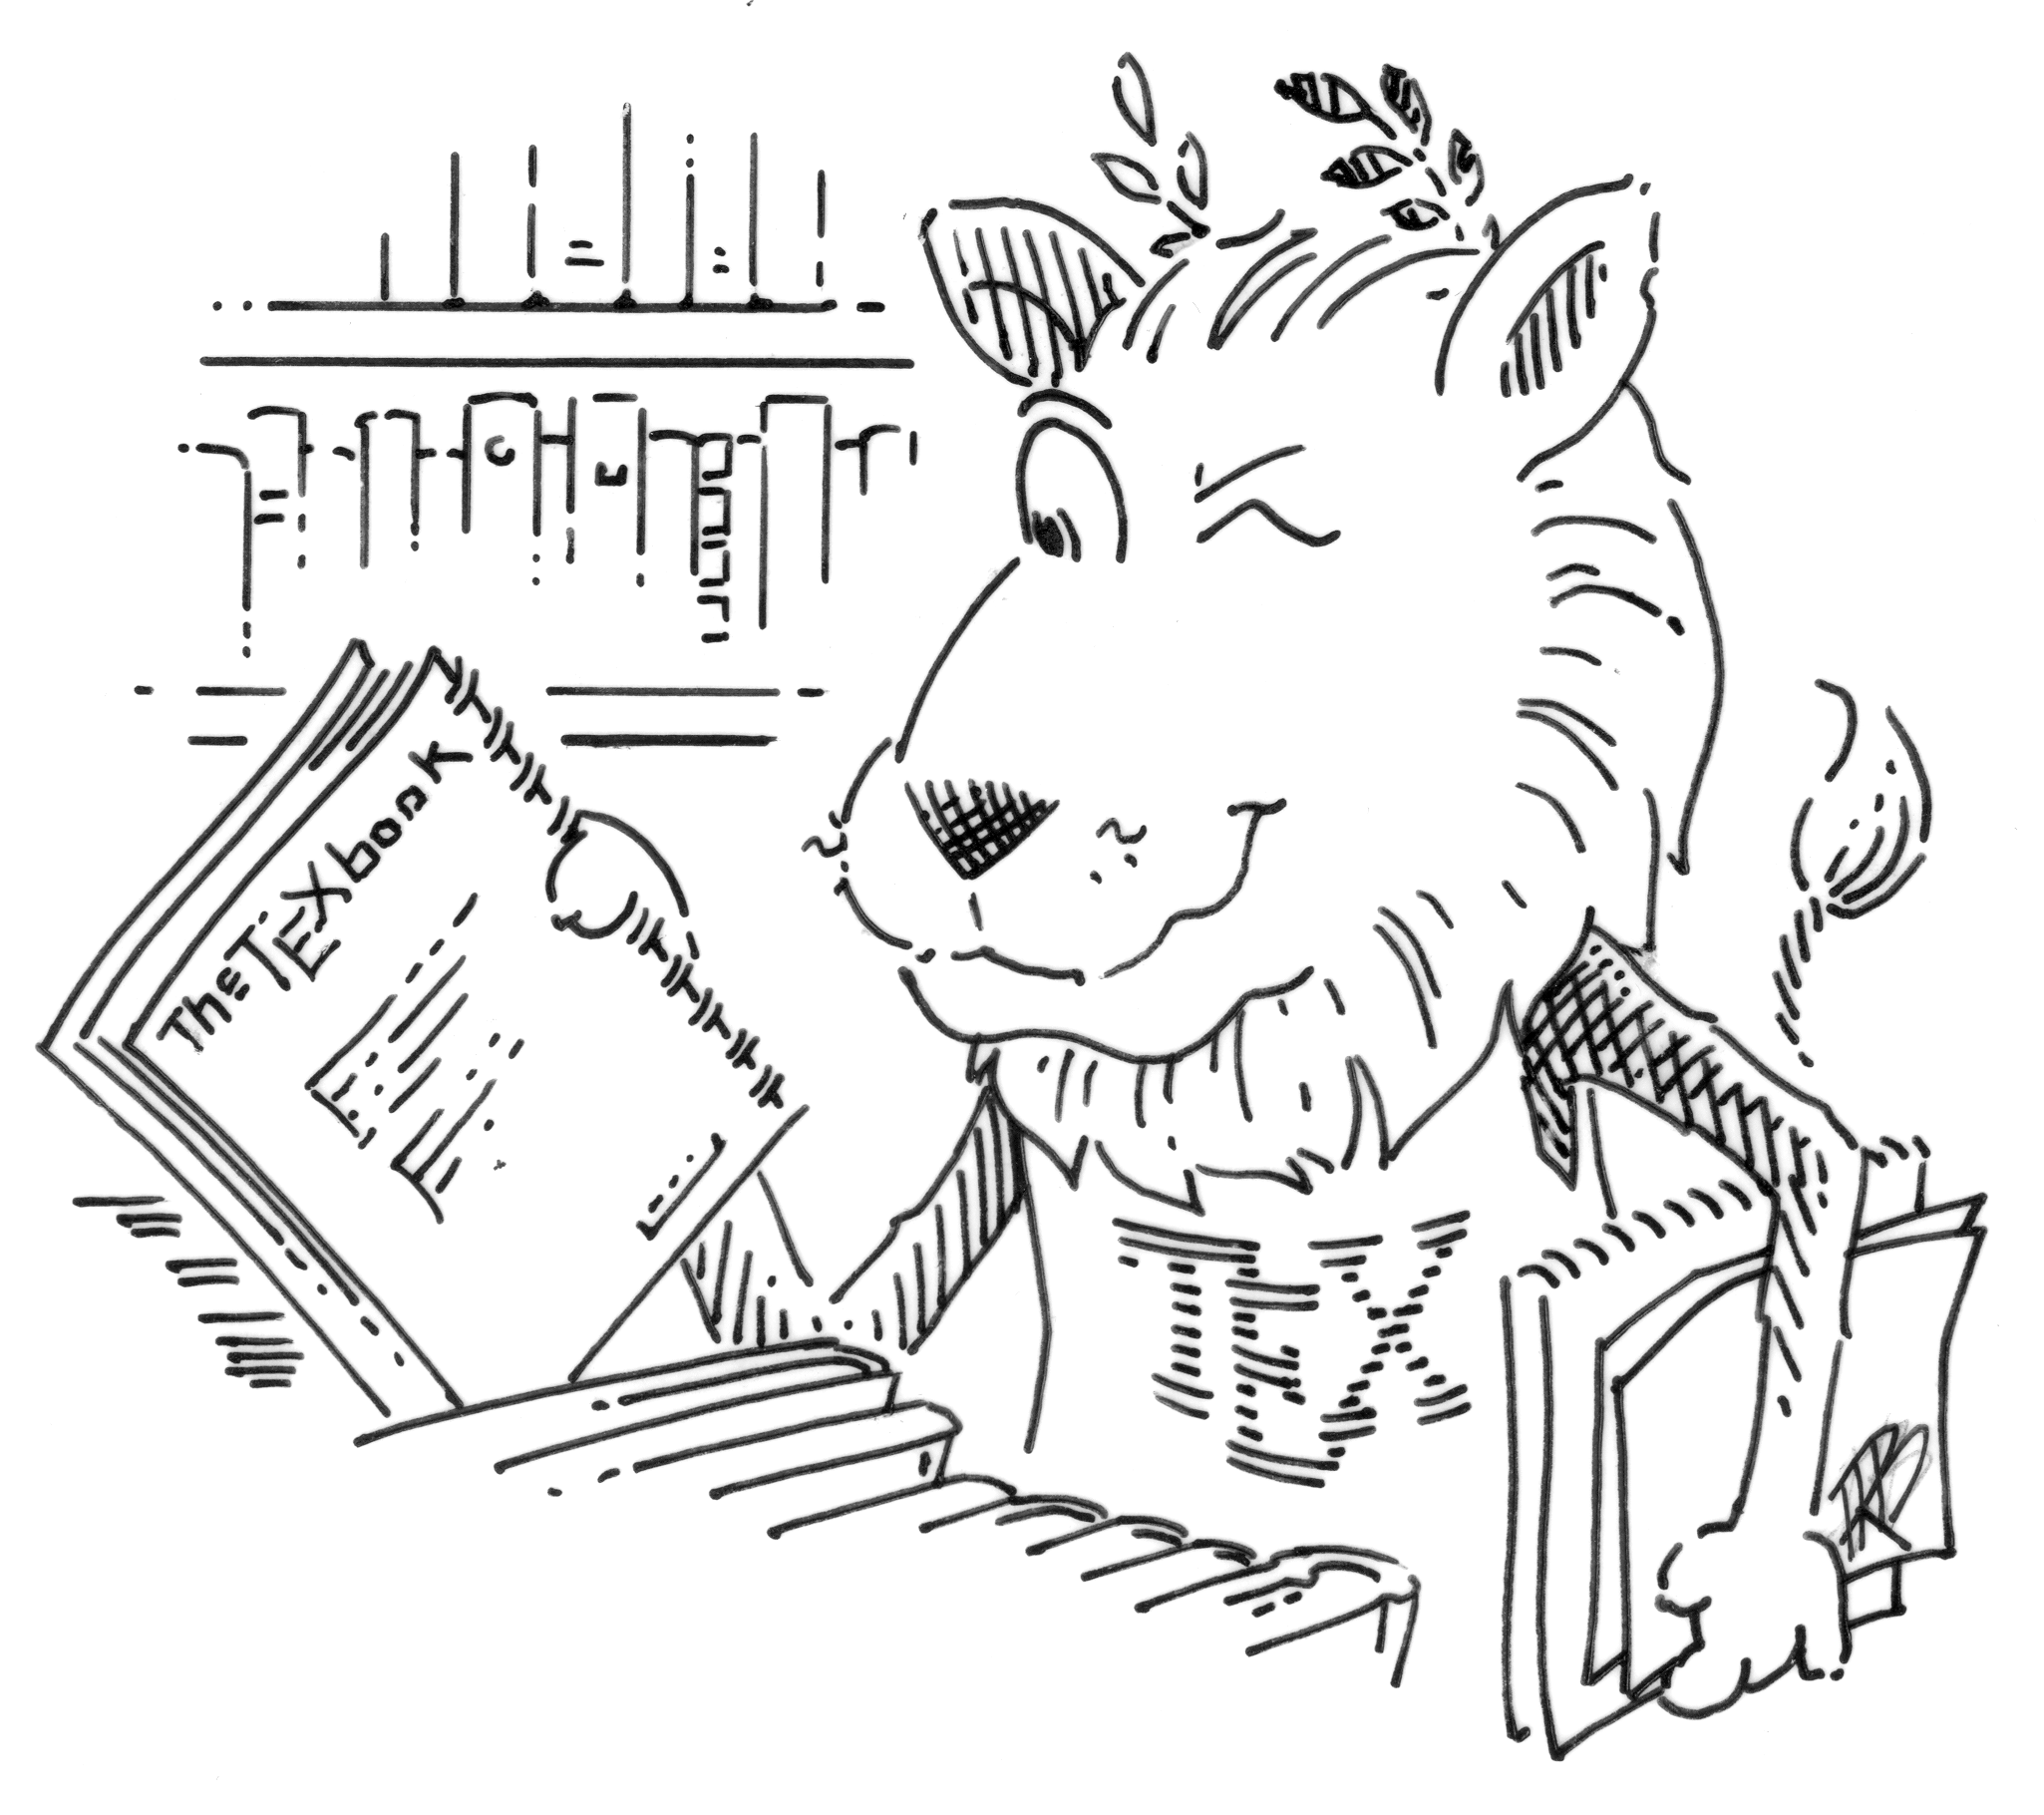
\includegraphics[width=0.4\linewidth]{figuras/tex_lion}
	\caption{Esto es una leyenda}
	\label{fig:texlion}
\end{figure}

Texto de primer párrafo. Lo vimos en la Figura \ref{fig:texlion} y en la Tabla \ref{tab:datos}.

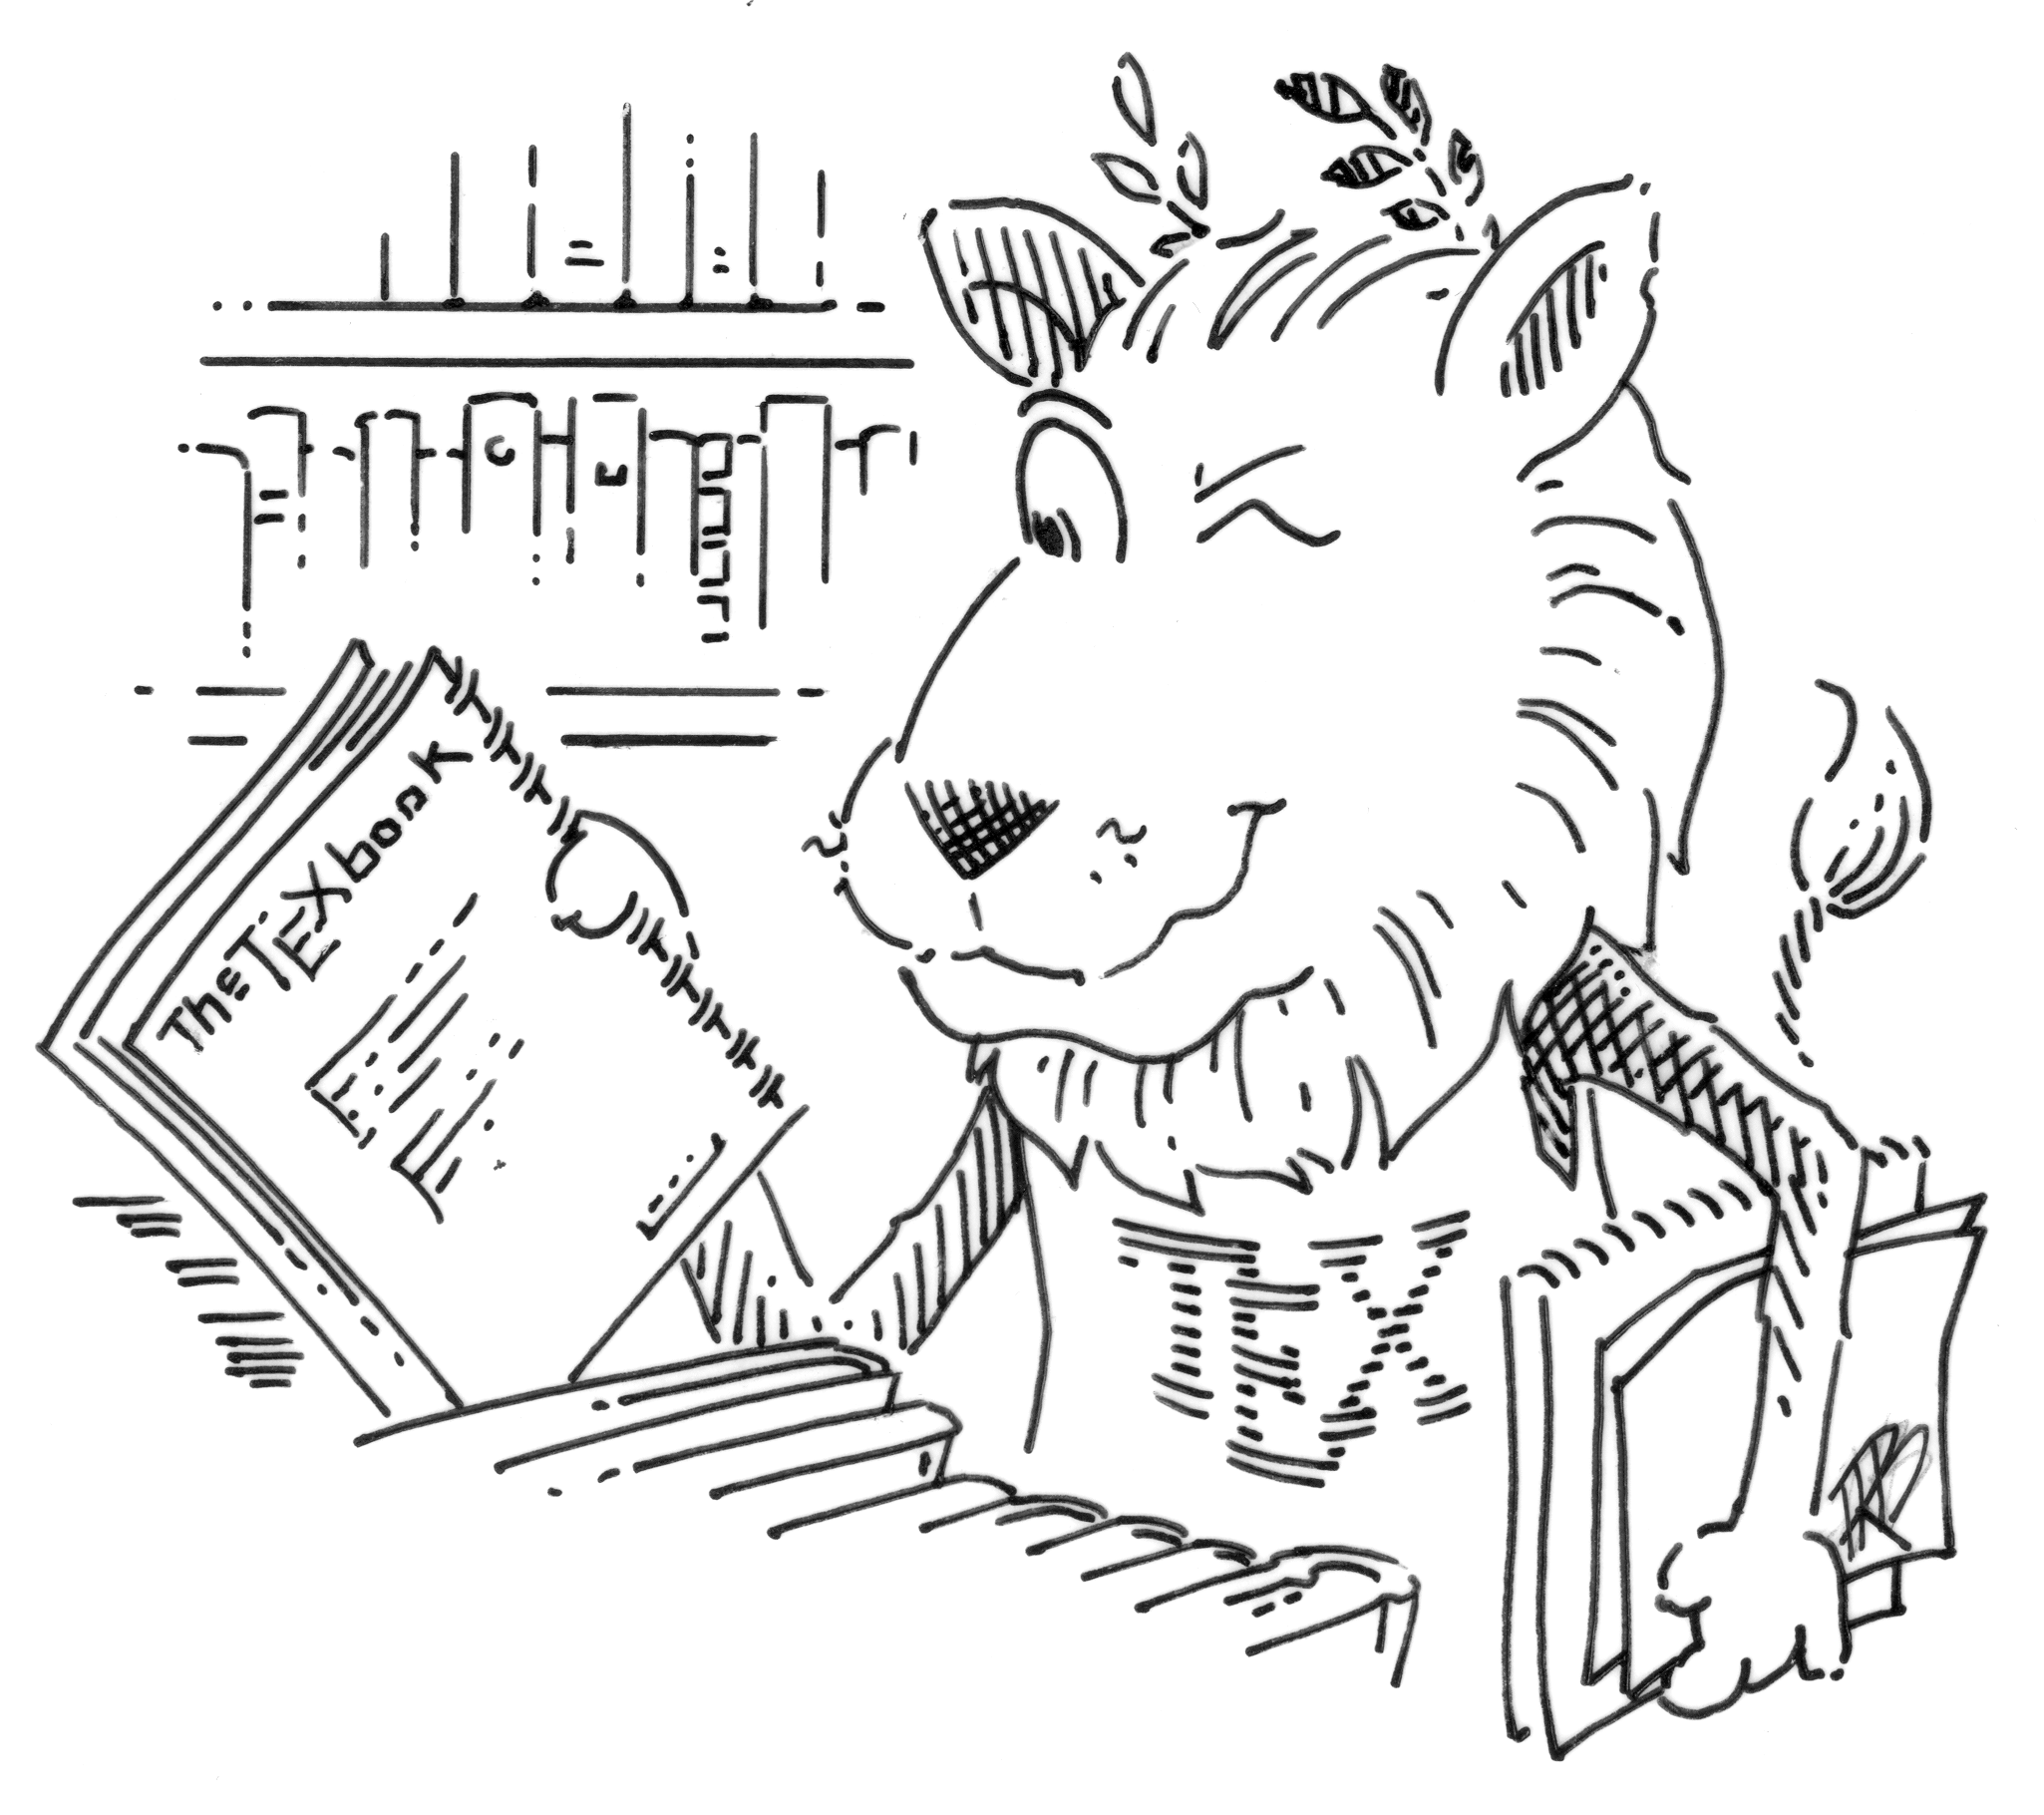
\includegraphics[width=0.4\linewidth]{figuras/tex_lion}

\begin{tabular}{|c|c|c|}
	\hline
	2 & 3 & 8 \\
	\hline
	4 & 2 & 5 \\
	\hline
	5 & 2 & hola \\
	\hline
\end{tabular}

\begin{table}[h]
	\centering
	\begin{tabular}{|c|c|c|}
		\hline
		2 & 3 & 8 \\
		\hline
		4 & 2 & 5 \\
		\hline
		5 & 2 & hola \\
		\hline
	\end{tabular}
	\caption{Esto es una tabla.}
	\label{tab:datos}
\end{table}

$$\underset{0}{\overset{L}{\int }}f\left(x\right)\cdot {x}^{2}\sum \bigvee=0$$

\end{document}
